% ----------------------------------------------------------
\chapter{Fundamentação Teórica}\label{cap:fundamentacaoTeorica}
% ----------------------------------------------------------
Esta seção apresenta os conceitos teóricos que sustentam o desenvolvimento do modelo preditivo para o nível do Lago Guaíba, com base em dados meteorológicos e na técnica de Regressão \textit{Ridge}. Inicialmente, aborda-se o impacto das mudanças climáticas e sua relação com eventos extremos, como as enchentes, destacando a relevância do monitoramento de rios em regiões vulneráveis, como o Rio Grande do Sul. Em seguida, são discutidos os princípios de aprendizado de máquina, com ênfase em abordagens supervisionadas, que formam a base para a modelagem proposta. Posteriormente, explora-se a teoria da regressão, incluindo a regressão linear simples e múltipla, e o método dos Mínimos Quadrados Ordinários, que são fundamentais para compreender a Regressão \textit{Ridge}. Por fim, detalha-se a técnica da regressão proposta para implementação, destacando sua capacidade de lidar com multicolinearidade e melhorar a generalização do modelo, essencial para a previsão precisa do nível do rio em cenários de alta variabilidade climática.

\section{As mudanças climáticas e as catástrofes naturais}

As grandes cidades brasileiras enfrentam desafios mais frequentes relacionados às mudanças climáticas, que agravam problemas como enchentes, inundações e deslizamentos. Projeções indicam que, até 2030, a mancha urbana de São Paulo pode aumentar em até 38\%, ampliando o risco para mais de 20\% das áreas de expansão urbana, que se tornarão suscetíveis a acidentes naturais. O aumento na frequência de eventos de chuvas intensas pode dobrar o número de dias com precipitação acima de 10 milímetros, agravando a vulnerabilidade da população, especialmente nas áreas periféricas e de menor infraestrutura \cite{Nobre2011}.

\subsection{Cenário de enchentes no sul do Brasil}

Com base no histórico das enchentes no Rio Grande do Sul, observa-se que os desastres relacionados ao excesso de chuvas não são um fenômeno recente. Desde 1941, o estado lida com eventos catastróficos, como a enchente que devastou Porto Alegre naquele ano, considerada uma das mais graves da história da cidade. Ao longo das décadas, esses episódios continuaram a ocorrer, expondo a vulnerabilidade da região diante de chuvas intensas e repentinas. A combinação de fatores naturais, como a geografia da região e os ciclos climáticos, aliado às ações humanas nocivas ao meio ambiente, contribui para a repetição e intensificação dessas tragédias \cite{veja2024}.

Em Santa Catarina, estado adjacente ao Rio Grande do Sul, as enchentes também são fenômenos recorrentes que, ao longo dos anos, têm causado impactos sociais, econômicos e ambientais. Um dos eventos mais recentes foi registrado em maio de 2024, quando o estado registrou vários dias com altos índices pluviométricos, levando ao transbordamento de rios, deslizamentos de terra e bloqueios em diversas rodovias \cite{g12024}.

\subsection{Dinâmica do Lago Guaíba}

O Lago Guaíba, principal manancial de abastecimento de água para a capital do Rio Grande do Sul e região, é alvo de estudo sobre diversos temas, incluindo sua hidrodinâmica e nível ao longo do ano. O Lago Guaíba apresenta flutuações significativas no volume de descarga, variando de 407 m³/s a 14.270 m³/s \cite{andrade2017}. Grande parte desta variação sofre influência dos rios que desemborcam no lago, como Rio Jacuí, que contribui com cerca de 84,6\% da água que aflui ao lago, além dos rios Sinos, Caí e Gravataí que contribuem com 7,5\%, 5,2\% e 2,7\%, respectivamente \cite{andrade2019}. 

Outro fator relevante em relação ao risco de enchentes do lago está no tempo de retenção das águas que chegam dos rios. Ao investigar os níveis de poluição do lago, devido a capital carecer de um tratamento de água 100\% efetivo, notou-se que grande parte da água do Guaíba fica retida por longos períodos, gerando baixa circulação e menor diluição de poluentes \cite{andrade2019}. Além do agravante da qualidade da água, esse comportamento faz com que o fluxo dos rios que chegam ao lago, em caso de um aumento atípico do volume, desencadeie enchentes que demoram para escoar, prejudicando ainda mais a população das cidades banhadas pelo lago. 

Na Figura \ref{fig:bacia_guaiba}, é mostrado alguns rios que fazem parte da bacia hidrográfica do Guaíba, e que influenciam diretamente no seu nível. À esquerda, percebe-se que um rio não é identificado, sendo este o Rio Jacuí, que contribui majoritariamente com o fluxo de água que aflui ao lago. Na Figura \ref{fig:bacia_guaiba_2}, fica evidente o motivo de seu maior impacto, dado sua extensão e largura maior que os demais rios. 

\begin{figure}[H]
	\caption{\label{fig:bacia_guaiba}Rios que desemborcam e influenciam no nível do Lago Guaíba.}
	\begin{center}
		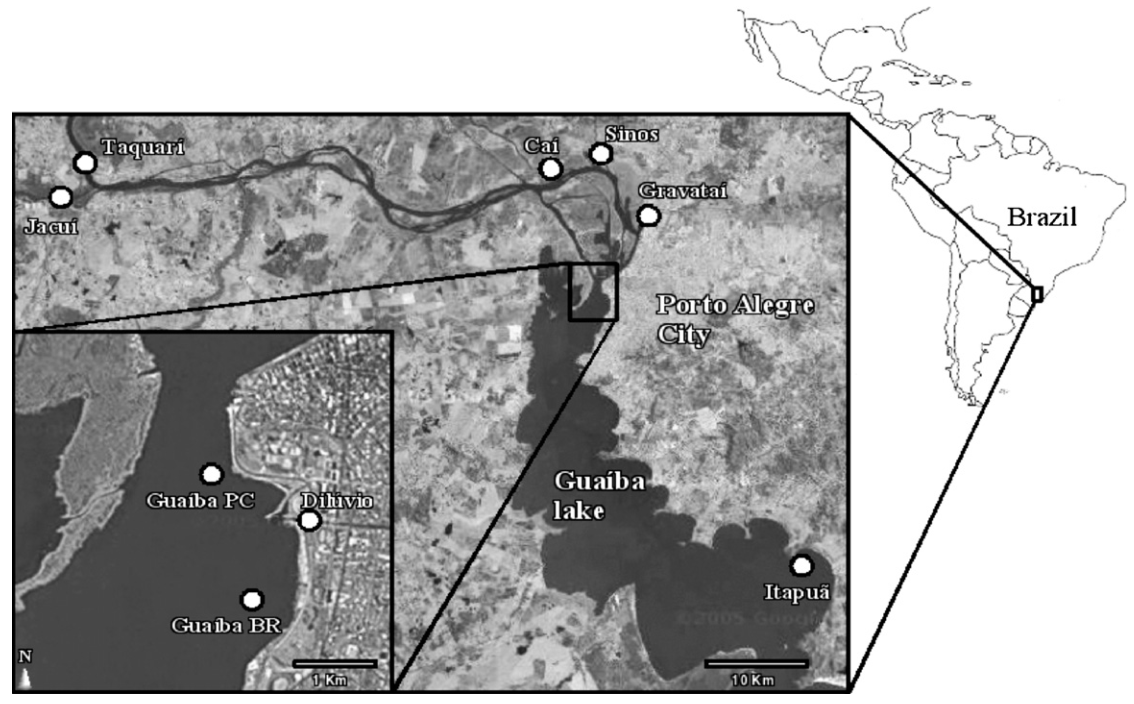
\includegraphics[scale=0.45]{figuras/bacia_lago_guaiba.png}
	\end{center}
	\fonte{\cite{g1_2024}.}
\end{figure}

\begin{figure}[H]
	\caption{\label{fig:bacia_guaiba_2}Rio Jacuí e seu desemboque no Lago Guaíba.}
	\begin{center}
		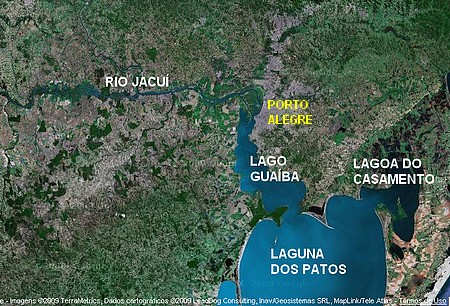
\includegraphics[scale=0.8]{figuras/lago_guaiba_2.jpg}
	\end{center}
	\fonte{\cite{portoimagem_2009}.}
\end{figure}

\section{Aprendizado de máquina}

Desde que os computadores foram inventados, criou-se o questionamento da possibilidade de fazê-los "pensar" de modo semelhante ao ser humano. Por meio desse avanço, diversas áreas sofreriam grandes transformações, uma vez que a capacidade da máquina aprender e aprimorar o seu conhecimento sobre determinado assunto traria melhorias e uma maior performance na atividade desejada \cite{carbonell1983}.

Embora os computadores ainda não alcancem o mesmo nível de aprendizado geral do ser humano, nos últimos anos, o \glsxtrfull{ML} se tornou realidade, com aplicações em diversos setores, agregando valor e conhecimento por meio de dados e informações antes tratados apenas por profissionais da área.

Esse conceito envolve a criação de sistemas que são capazes de aprender a partir de dados, identificando padrões e realizando previsões sem a necessidade de programação explícita. O principal objetivo do \gls{ML} é construir algoritmos que permitam que os computadores adquiram conhecimento e melhorem sua performance de forma autônoma, baseando-se em experiências passadas \cite{carbonell1983}.

\subsection{Categorias de aprendizado de máquina}

Os quatro principais tipos de \gls{ML} são: supervisionado, não supervisionado, semi-supervisionado e reforço \cite{saravanan2018}. Estes tipos de \gls{ML} são descritos a seguir:

\begin{itemize}
    \item Supervisionado: envolve a utilização de dados rotulados, no qual o modelo é treinado com entradas e saídas conhecidas para fazer previsões sobre novos dados;
    \item Não supervisionado: lida com dados não rotulados, onde o sistema busca encontrar padrões ou agrupamentos nos dados;
    \item Semissupervisionado: combina elementos de ambos os métodos, utilizando uma pequena quantidade de dados rotulados e uma grande quantidade de dados não rotulados, sendo útil em cenários onde a rotulação de dados é cara ou complexa;
    \item Aprendizado por reforço: se baseia em um sistema de recompensas e punições, onde o sistema interage com o ambiente e aprende a otimizar suas ações para alcançar um objetivo a partir de \textit{feedbacks} recebidos.
\end{itemize}

\section{Regressão}
\label{sec:regressao}

\hl{Para prever e entender a dinâmica de fenômenos estudados, a regressão, uma técnica de aprendizado supervisionado, modela relações entre variáveis dependentes e independentes por meio de métodos estatísticos} \cite{soto2013}.

Em uma equação linear, uma variável independente, comumente representada pela letra $x$, caracteriza uma grandeza que está sendo manipulada durante um experimento. Dado esse comportamento, a variável $x$ não sofre influência de outras variáveis. A variável dependente, comumente representada pela letra $y$, caracteriza valores que estão diretamente associados à variável independente. Assim, de forma direta ou indireta, $x$ exerce influência sobre $y$.

A Figura \ref{fig:regressao_exemplo} ilustra um exemplo de regressão, mostrando a relação entre o índice de felicidade e a expectativa de vida em diversos países, conforme dados de \cite{helliwell2020}. Nesse contexto, o índice de felicidade é considerado a variável independente, enquanto a expectativa de vida é a variável dependente. Observando o gráfico, é possível perceber uma tendência de que países com maior índice de felicidade apresentam também uma expectativa de vida mais elevada. Assim, a regressão busca ajustar uma reta que, de forma aproximada, modela essa relação entre as variáveis, permitindo estimar valores de expectativa de vida a partir de valores do índice de felicidade. Tal reta pode ser representada pela equação linear mencionada anteriormente, e, caso disponível, a equação gerada pelos dados pode ser informada para descrever matematicamente a tendência observada na figura.

\begin{figure}[H]
	\caption{\label{fig:regressao_exemplo}Relação entre o índice de felicidade e expectativa de vida.}
	\begin{center}
		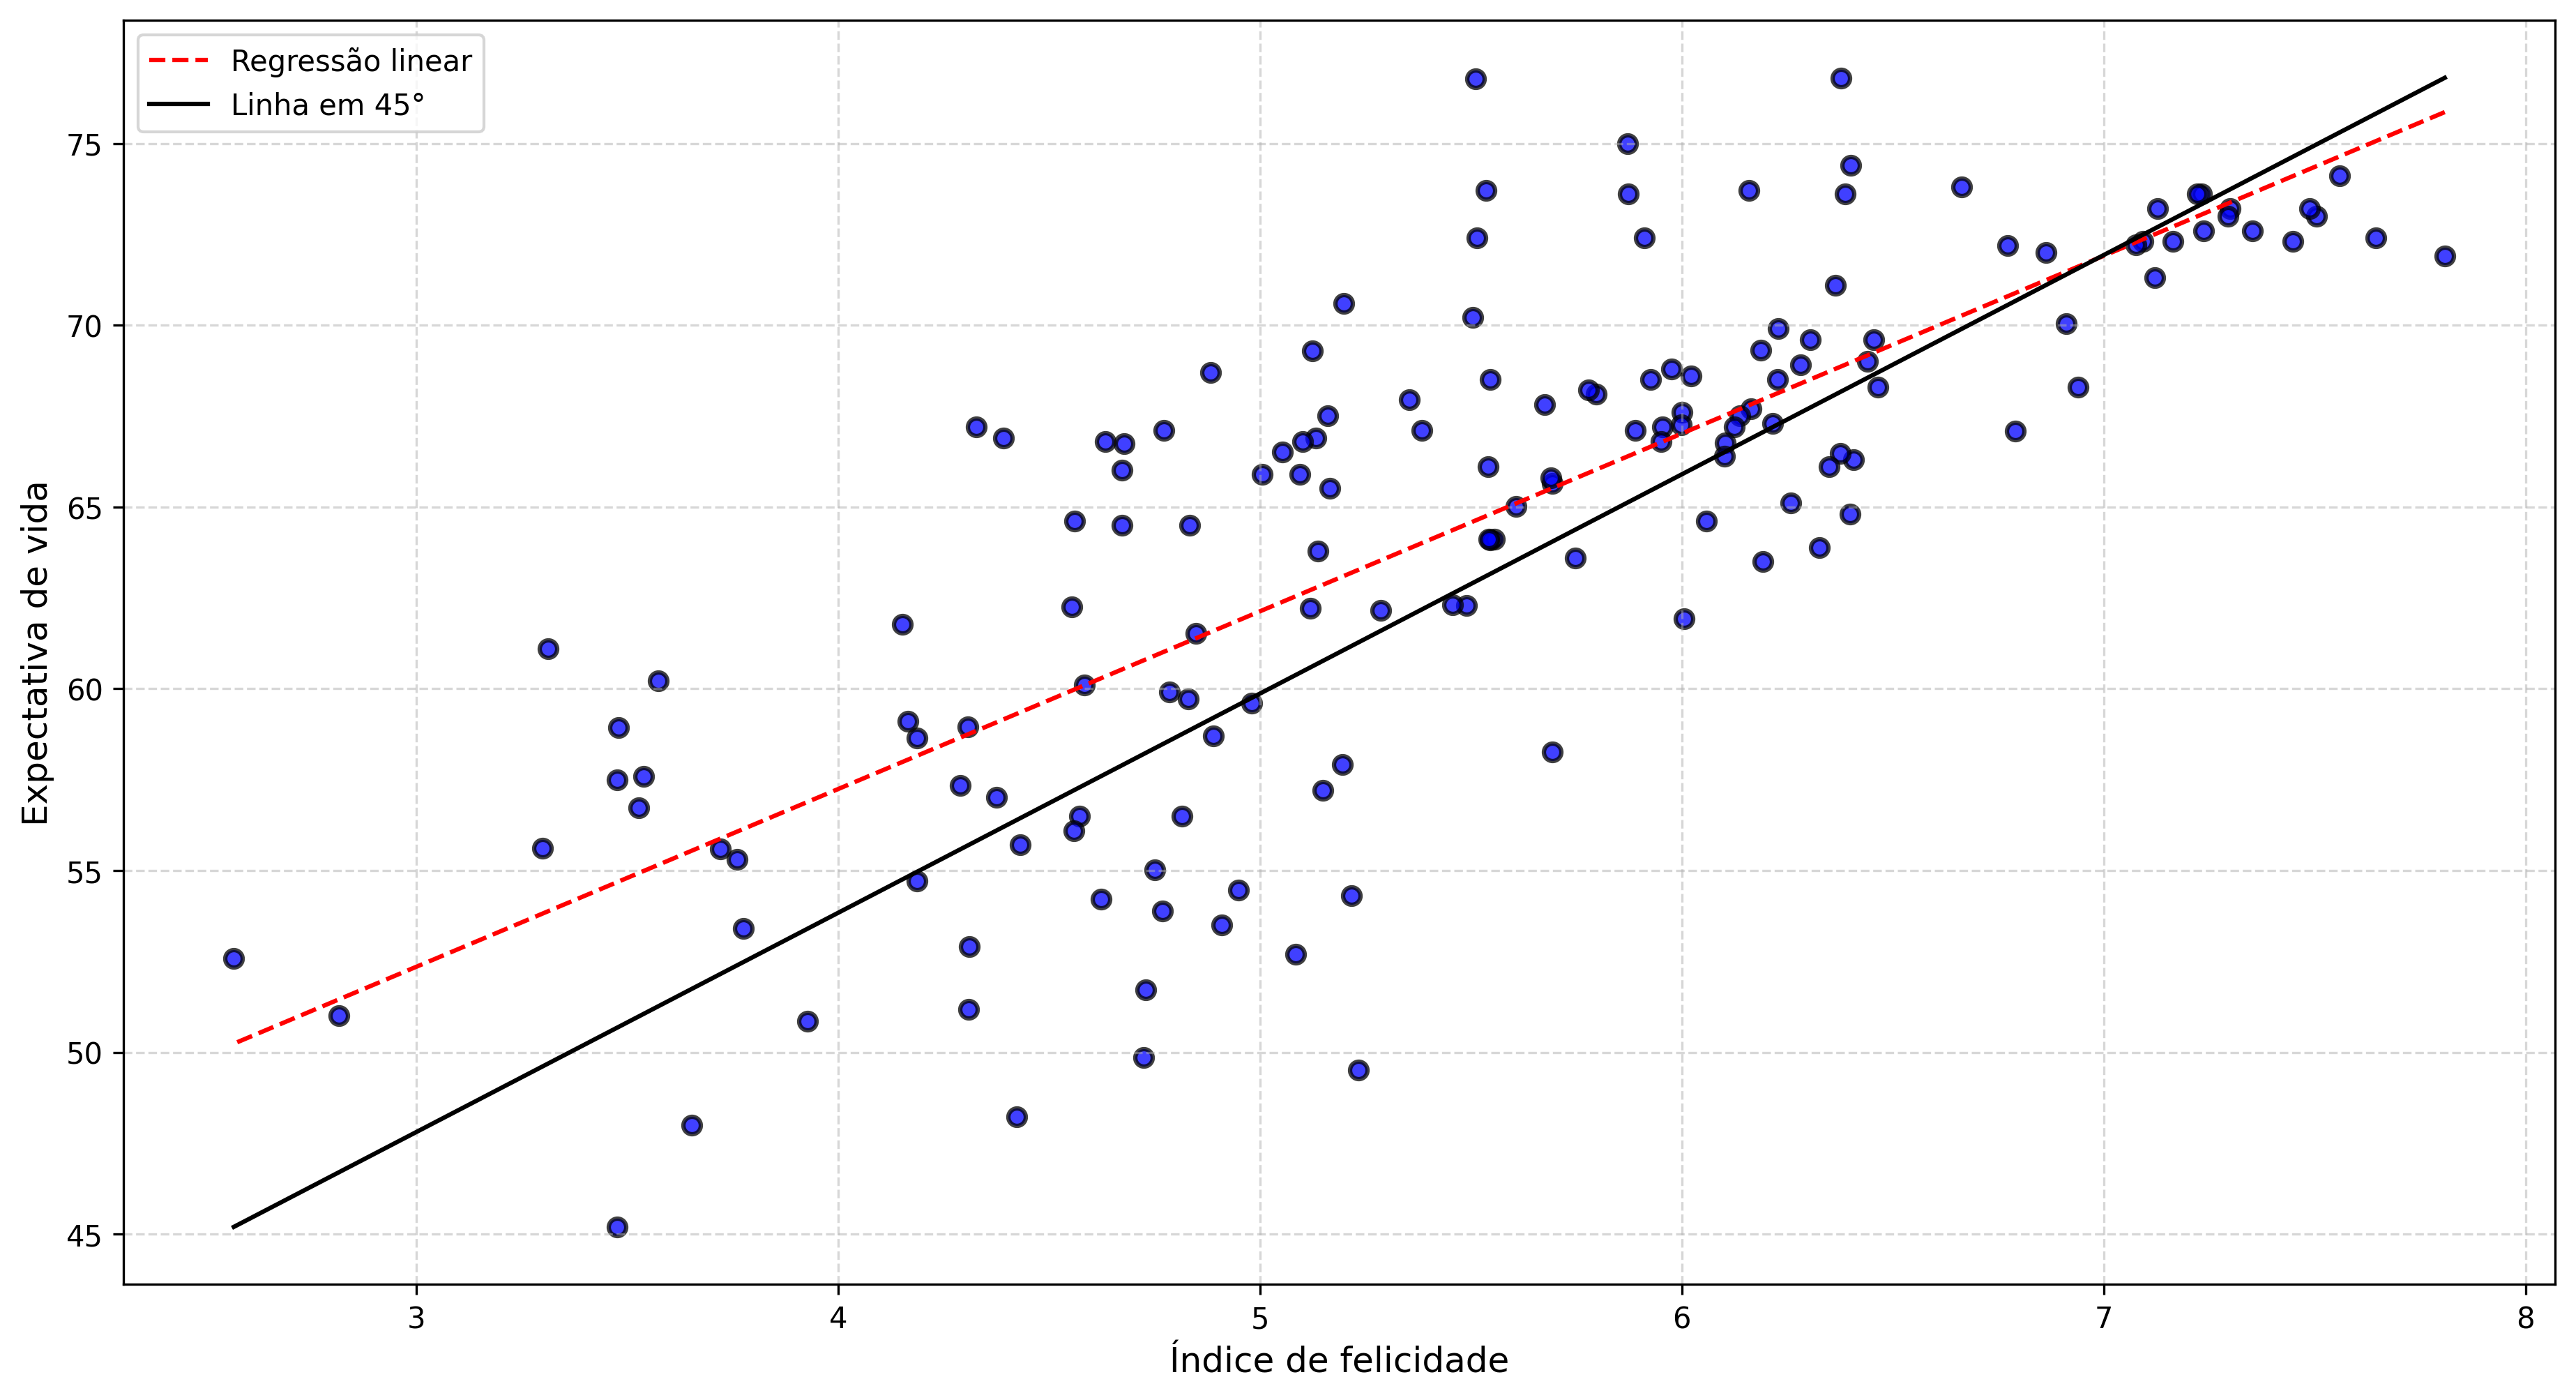
\includegraphics[scale=0.4]{figuras/happiness_world.png}
	\end{center}
	\fonte{\cite{helliwell2020}}
\end{figure}

Embora uma inferência inicial permita constatar uma correlação entre as variáveis da equação, a criação de um modelo de previsão necessita de métodos que comprovem a correlação pressuposta. Para determinar as relações entre as variáveis dependentes e independentes de um sistema, coeficientes de correlação são calculados, gerando valores que medem e comprovam estatisticamente o grau de correspondência dos fatores estudados. Uma das métricas de correlação mais utilizadas é o coeficiente de Pearson, que mede a associação linear entre duas variáveis \cite{kirch2008}. 

Esse coeficiente de correlação pode ser definido pela Equação \ref{eq:correlacao_person}, onde $n$ é o total de amostras, $\bar{x}$ e $\bar{y}$ são as médias aritméticas de ambas as variáveis. Os valores do coeficiente de Pearson variam entre -1 e 1, de tal forma que quanto mais próximos desses extremos, melhor correlacionadas estão as variáveis.

\begin{equation}
    r_{xy} = \frac{\sum_{i=1}^n (x_i - \bar{x})(y_i - \bar{y})}{\sqrt{\sum_{i=1}^n (x_i - \bar{x})^2 \sum_{i=1}^n (y_i - \bar{y})^2}}
    \label{eq:correlacao_person}
\end{equation}

A Figura \ref{fig:correlacoes} mostra alguns exemplos com gráficos de dispersão de variáveis com diferentes correlações.

\begin{figure}[H]
	\caption{\label{fig:correlacoes}Diferentes correlações entre variáveis.}
	\begin{center}
		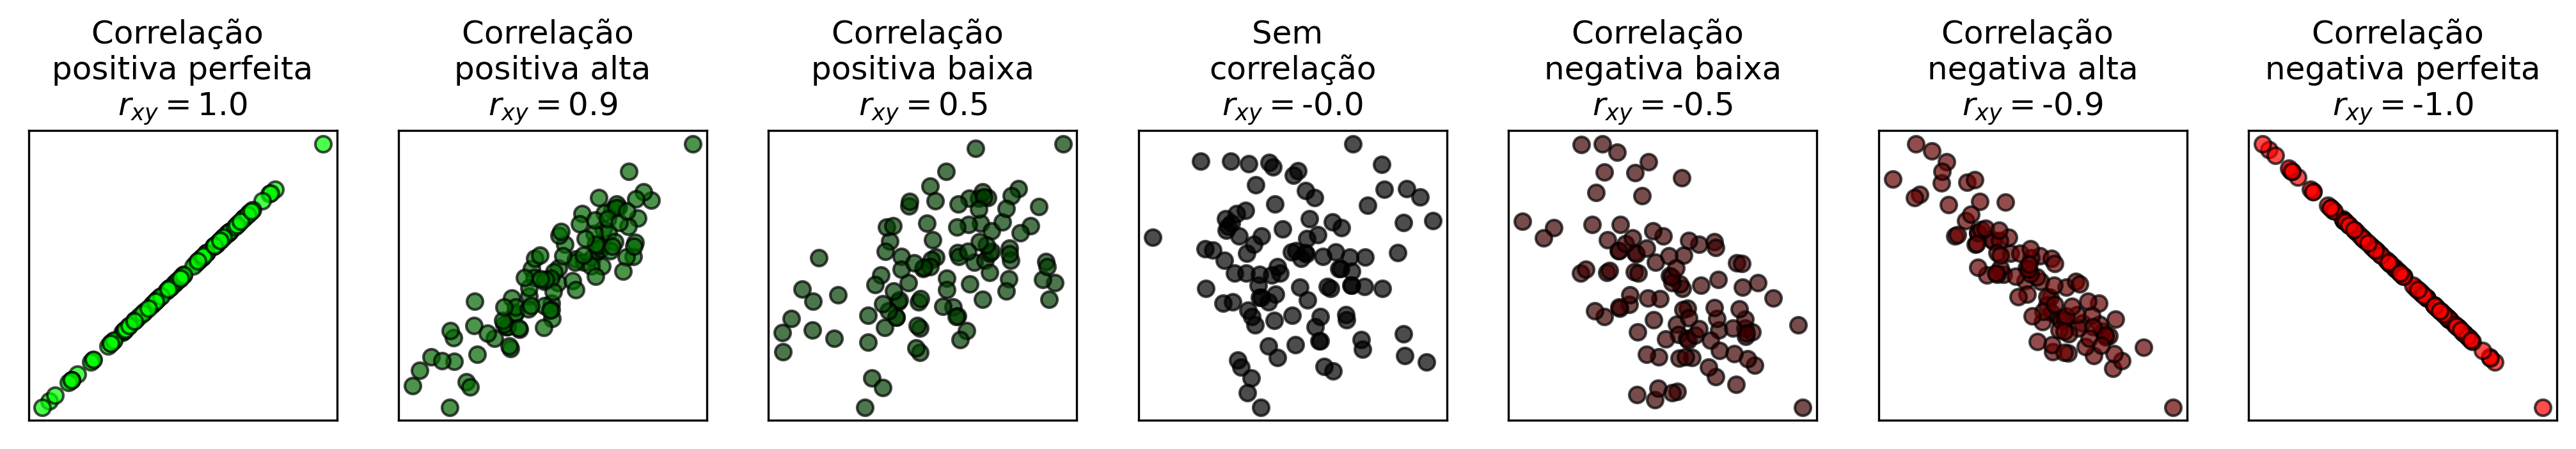
\includegraphics[scale=0.4]{figuras/correlations.png}
	\end{center}
	\fonte{\cite{helliwell2020}}
\end{figure}

Quando o coeficiente de correlação indica uma alta correlação entre variáveis independentes (por exemplo, dados meteorológicos) e a variável dependente (nível do Lago Guaíba), métodos mais simples de regressão podem ser utilizados para estimar valores não presentes no conjunto de dados, aproveitando a relação estatística identificada. No entanto, em casos onde o coeficiente indica baixa correlação entre as variáveis ou alta multicolinearidade entre as preditoras, métodos como a regressão Ridge se mostram vantajosos, pois incorporam uma penalidade (regularização L2) que reduz o impacto de variáveis menos relevantes ou correlacionadas, permitindo previsões mais robustas sem depender exclusivamente da força da correlação linear.

\section{Regressão Linear}
\label{sec:regressao-linear}

A regressão linear é um tipo específico de regressão que modela a relação entre uma variável independente e uma variável dependente, conforme citado em \ref{sec:regressao}. Amplamente utilizada em áreas como engenharia, ciências físicas, economia e ciências sociais, essa técnica assume que a relação entre as variáveis é linear, permitindo prever valores da variável dependente com base em uma ou mais variáveis independentes \cite{montgomery2012}.

A aplicação da técnica é relevante devido à sua simplicidade e capacidade de fornecer previsões baseadas em uma fórmula matemática interpretável. Além disso, o método é base para implementações de algoritmos na área de ciência de dados, otimizando o processamento de dados complexos e viabilizando a criação de modelos de previsão \cite{aws2024}.

O método de regressão linear é dividido em dois grupos, sendo eles: \glsxtrfull{RLS} e \glsxtrfull{RLM} \cite{montgomery2012}. A RLS tem como objetivo estabelecer uma relação entre duas variáveis através de uma função, cuja definição é dada por:

\begin{equation}
	y = \beta_0 + \beta_1 x + \varepsilon
	\label{eq:regressao_linear_simples}
\end{equation}

Onde $y$ é a variável dependente, $x$ a variável independente, enquanto $\beta_0$ e $\beta_1$ são coeficientes calculados pela regressão, que representam o valor de $y$ quando $x=0$ e o grau de inclinação da reta, respectivamente.

A RLM, embora seja semelhante à RLS, possui múltiplas variáveis preditoras, sendo definida por:

\begin{equation}
	y = \beta_0 + \beta_1 x_{1} + \beta_2 x_{2} + ... + \beta_k x_{k} + \varepsilon
	\label{eq:regressao_linear_multipla}
\end{equation}

Na equação \ref{eq:regressao_linear_multipla}, $y$ é a variável alvo, $x_{1}$ a $x_{k}$ as variáveis regressoras, e $\beta_0$ permanece sendo o coeficiente de intercepto do eixo Y enquanto $\beta_1$ a $\beta_n$ representam os coeficientes associados à n-ésima variável \cite{sassi2012}.

Nas equações \ref{eq:regressao_linear_simples} e \ref{eq:regressao_linear_multipla}, nota-se a presença do erro estatístico representado por $\varepsilon$, que é a diferença entre o valor observado e o valor previsto pela equação de regressão. Esse erro é considerado aleatório e contabiliza a falha do modelo ao tentar se aproximar do comportamento denotado pelos dados amostrados \cite{montgomery2012}.

Para compreender o modelo de regressão linear sob suas suposições fundamentais, considera-se que a variável independente $ x $ (por exemplo, precipitação meteorológica) é conhecida e usada para prever a variável dependente $ y $ (como o nível do Lago Guaíba). Sob essas condições, todos os termos do lado direito da equação $ y = \beta_0 + \beta_1 x + \varepsilon $ são conhecidos, exceto o erro $ \varepsilon $, que determina as propriedades estatísticas de $ y $. Assumindo que o erro $ \varepsilon $ tem média zero e variância constante $ \sigma^2 $ \cite{montgomery2012}, a resposta média para qualquer valor de $ x $ é dada por

\begin{equation}
	E(y \mid x) = \mu_{y \mid x} = E(\beta_0 + \beta_1x + \varepsilon) = \beta_0 + \beta_1x
\end{equation}

e a variância é dada por:

\begin{equation}
	Var (y \mid x) = \sigma_{y \mid x}^2 = Var(\beta_0 + \beta_1x + \varepsilon) = \sigma^2
\end{equation}

Desse modo, o modelo de regressão verdadeiro $\mu_{y \mid x} = \beta_0 + \beta_1x$ representa uma linha de valores médios, ou seja, a altura da linha de regressão em qualquer valor de x corresponde ao valor esperado de y para aquele x.

Para exemplificar as suposições da regressão linear, considera-se um modelo ilustrado pela Figura 3a, onde a média condicional é $ \mu_{y|x} = 3.5 + 2x $ e a variância do erro é $ \sigma^2 = 2 $. O erro $ \varepsilon $ segue uma distribuição normal, descrevendo a variação aleatória em torno da média. Como $ y $ é a soma de uma componente linear $ \beta_0 + \beta_1 x $ (a média) e o erro $ \varepsilon $, normalmente distribuído, $ y $ também segue uma distribuição normal. Por exemplo, para um valor específico da variável independente $ x = 10 $, $ y $ terá uma distribuição normal com média $ \mu_{y|x} = 3.5 + 2(10) = 23.5 $ e variância $ \sigma^2 = 2 $. Quanto menor a variância, mais próximos os pontos estarão da linha de regressão; uma variância maior resulta em maior dispersão em relação à linha de regressão \cite{montgomery2012}.

A maioria dos fênomenos nos quais se deseja obter a função que descreve o seu comportamento resulta em uma aproximação funcional através das variáveis de interesse. Essas relações funcionais frequentemente baseiam-se em teorias físicas, químicas ou de engenharia e ciências, ou seja, no conhecimento do mecanismo subjacente. Na Figura \ref{fig:regressao_linear_aprox_relacao_complexa}, é mostrada uma relação entre as variáveis $x$ e $y$ relativamente complexa, mas que pode ser aproximada de por uma equação de regressão linear, com um erro relativamente baixo.

\begin{figure}[H]
	\centering
	\caption{Interpretação de uma regressão linear}
	\begin{subfigure}{0.4\textwidth}
	  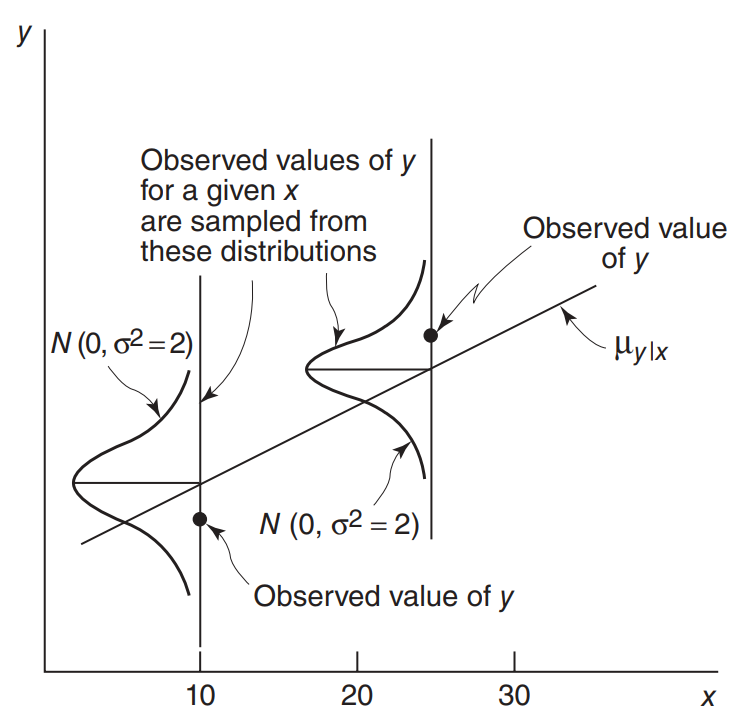
\includegraphics[width=\linewidth]{figuras/how_observations_are_generated_in_linear_regression.png}
	  \caption{Como as observações são geradas na regressão linear}
	  \label{fig:observacoes_regressao_linear}
	\end{subfigure}
	\hspace{0.5cm}
	\begin{subfigure}{0.4\textwidth} 
		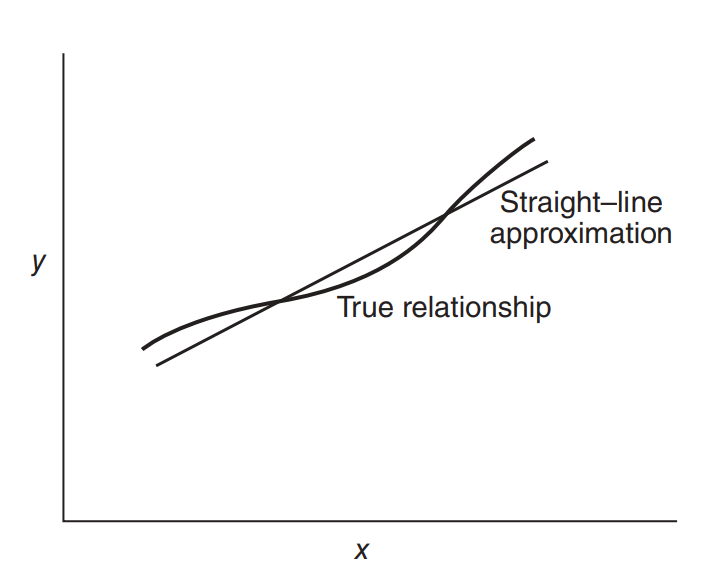
\includegraphics[width=\linewidth]{figuras/linear_regression_approximation_of_a_complex_relationship.png}
		\caption{Regressão linear como aproximação de uma relação complexa}
		\label{fig:regressao_linear_aprox_relacao_complexa}
	\end{subfigure}
	\label{fig:comportamento_regressao_linear}
	\fonte{\cite{montgomery2012}}
\end{figure}

Contudo, em alguns casos, quando a dinâmica do modelo a ser estimada passa a ter um grau de complexidade maior, como é o caso da Figura \ref{fig:aproximacao_linear_complexa}, utlizar uma RLS pode implicar em erros que extrapolam a tolerância exigida no estudo. Nesses cenários, utilizar uma função de regressão linear em intervalos específicos, ou seja, uma RLM, se torna uma alternativa plausível, tendo em vista que, para intervalos menores onde a dinâmica do fênômeno é mais linear, a regressão apresenta um erro menor, como mostra a Figura \ref{fig:intervalo_aplicacao_rls}.

\begin{figure}[H]
	\centering
	\caption{Situações de inadequação da RLS}
	\begin{subfigure}{0.4\textwidth}
	  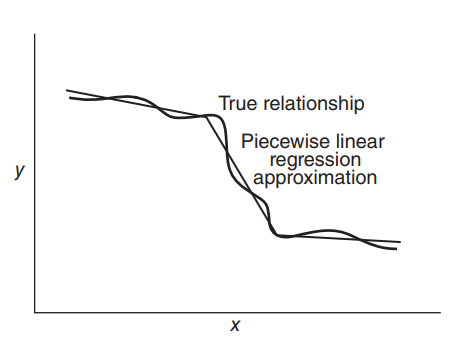
\includegraphics[width=\linewidth]{figuras/piecewise_linear_approximation.png}
	  \caption{Aproximação Linear complexa}
	  \label{fig:aproximacao_linear_complexa}
	\end{subfigure}
	\hspace{0.5cm}
	\begin{subfigure}{0.4\textwidth} 
		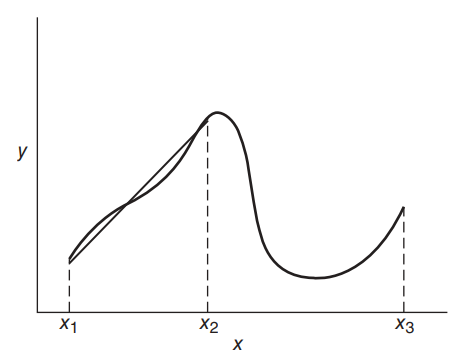
\includegraphics[width=\linewidth]{figuras/danger_extrapolation_regression.png}
		\caption{Intervalo de aplicação da RLS}
		\label{fig:intervalo_aplicacao_rls}
	\end{subfigure}
	\label{fig:comportamento_regressao_linear}
	\fonte{\cite{montgomery2012}}
\end{figure}

Partindo desses conceitos, para implementação de modelos de regressão linear e múltipla, o método dos Mínimos Quadrados Ordinários se apresenta como uma abordagem para estimar a melhor regressão dos pontos observados, encontrando uma reta com o menor erro entre as amostras e os valores da função estudada.

\section{Método dos quadrados ordinários}

O método \glsxtrfull{MQO} atua como uma ferramenta estatística, visando estimar a relação entre uma variável dependente e uma ou mais variáveis independentes \cite{Alkama2020}, permitindo encontrar os coeficientes desejados para o funcionamento do modelo.

\hl{Para obter uma regressão que se aproxima da dinâmica analisada, o método visa minimizar a} \glsxtrfull{RSS}\hl{, denotado pela equação} \ref{eq:rss_rls} \hl{para os casos de RLS (isto é, quando há apenas uma variável independente)}.

\begin{equation}
	RSS = \sum_{i=1}^{n} \left(y_i - \beta_0 - \beta_1x_{i}\right)^2
	\label{eq:rss_rls}
\end{equation}

Para o caso de \gls{RLM}, utiliza-se a equação \ref{eq:rss_rlm}, onde:

\begin{itemize}
    \item $y_i$ é uma variável aleatória e representa o valor da variável resposta (variável dependente) na i-ésima observação
    \item $x_{ij}$ representa o valor da j-ésima variável explicativa (variável independente, variável regressora) na i-ésima observação. Nota-se que podem existir $p$ variáveis independentes (sendo $p \geq 1$) para uma variável independente; 
    \item $\beta_{0}$ e $\beta_{j}$ são os parâmetros do modelo que serão estimados, e que definem a reta de regressão
\end{itemize}

\begin{equation}
    RSS = \sum_{i=1}^{n} \left(y_i - \beta_0 - \sum_{j=1}^{p}\beta_jx_{ij}\right)^2
	\label{eq:rss_rlm}
\end{equation}

Para minimizar a SSR em um caso de RLS, por exemplo, são calculadas as derivadas parciais de $\beta_0$ e $\beta_1$, igualando ambas a zero.

Derivada em relação à $\beta_0$:

\begin{equation}
	\frac{\partial RSS}{\partial \beta_0} = -2 \sum_{i=1}^n (y_i - \beta_0 - \beta_1 x_i) = 0
\end{equation}

simplificando:

\begin{gather*}
	\sum_{i=1}^n (y_i - \beta_0 - \beta_1 x_i) = 0 \\
	\sum_{i=1}^n y_i - n \beta_0 - \beta_1 \sum_{i=1}^n x_i = 0
\end{gather*}

divindindo por $n$:

\begin{gather*}
	\frac{\sum_{i=1}^n y_i}{n} - \beta_0 - \beta_1 \frac{\sum_{i=1}^n x_i}{n} = 0 \\
	\bar{y} - \beta_0 - \beta_1 \bar{x} = 0
\end{gather*}

onde $\bar{y}$ e $\bar{x}$ são as médias amostrais de $y$ e $x$, respectivamente. Assim, a equação pode ser reescrita como:

\begin{equation}
	\beta_0 = \bar{y} - \beta_1 \bar{x}
	\label{eq:beta0}
\end{equation}

Derivada em relação à $\beta_1$:

\begin{equation}
	\frac{\partial SSR}{\partial \beta_1} = -2 \sum_{i=1}^n x_i (y_i - \beta_0 - \beta_1 x_i) = 0
\end{equation}

substituindo $\beta_0$ na equação:


\begin{gather*}
	\sum_{i=1}^n x_i (y_i - (\bar{y} - \beta_1 \bar{x}) - \beta_1 x_i) = 0 \\
	\sum_{i=1}^n x_i (y_i - \bar{y} + \beta_1 \bar{x} - \beta_1 x_i) = 0 \\
	\sum_{i=1}^n x_i (y_i - \bar{y}) + \sum_{i=1}^n x_i (\beta_1 \bar{x} - \beta_1 x_i) = 0 \\
	\sum_{i=1}^n x_i (y_i - \bar{y}) - \beta_1 \sum_{i=1}^n x_i (x_i - \bar{x}) = 0
\end{gather*}

sabendo que:

\begin{gather*}
	\sum_{i=1}^n x_i (x_i - \bar{x}) = \sum_{i=1}^n (x_i - \bar{x})^2
\end{gather*}

e

\begin{gather*}
	\sum_{i=1}^n x_i (y_i - \bar{y}) = \sum_{i=1}^n (x_i - \bar{x})(y_i - \bar{y})	
\end{gather*}

portanto:

\begin{gather*}
	\sum_{i=1}^n (x_i - \bar{x})(y_i - \bar{y}) = \beta_1 \sum_{i=1}^n (x_i - \bar{x})^2
\end{gather*}

\begin{equation}
	\beta_1 = \frac{\sum_{i=1}^n (x_i - \bar{x})(y_i - \bar{y})}{\sum_{i=1}^n (x_i - \bar{x})^2}
\end{equation}




Desse modo, a partir de um problema onde uma ou mais entradas geram amostras que resultam em uma saída, torna-se possível estimar uma função que melhor representa seu comportamento, minimizando ao máximo o valor da soma residual dos quadrados entre os pontos amostrais e a curva do modelo. 

\begin{table}[h!]
\centering
\begin{tabular}{|c|c|}
\hline
\textbf{Variável Independente} & \textbf{Variável Dependente} \\
\hline
0,38 & 6,98 \\
0,41 & 4,05 \\
0,44 & 5,52 \\
0,59 & 6,93 \\
0,98 & 6,57 \\
1,04 & 6,41 \\
1,22 & 8,27 \\
1,53 & 6,93 \\
1,74 & 8,89 \\
1,84 & 9,31 \\
\hline
\end{tabular}
\caption{Tabela de Valores Ordenados: Variável Independente vs. Variável Dependente}
\label{tab:valores_exemplo_mqo}
\end{table}

A Tabela \ref{tab:valores_exemplo_mqo} apresenta um exemplo de dados amostrais, onde a variável independente é representada pela primeira coluna e a variável dependente pela segunda coluna. A partir desses dados, é possível aplicar o método dos mínimos quadrados para encontrar os coeficientes que melhor se ajustam à reta de regressão linear.

Ao aplicar o método para resolver um problema, como é o caso da Tabela \ref{tab:valores_exemplo_mqo}, todos os pontos amostrados são utilizados para encontrar a reta que melhor se ajusta aos dados. Contudo, visando mostrar como a dinâmica de regressão utilizando MQO funciona, nos passos seguintes, as amostras são consideradas de forma cumulativa, alterando a cada iteração os valores de $\beta_0$ e $\beta_1$, até que a reta de regressão linear se ajuste aos dados amostrais.

Passo 1: Apenas o ponto (0.44, 5.52)

Com um único ponto, a reta passa exatamente por sobre o mesmo, porém o método MQO exige pelo menos dois pontos para definir uma inclinação. Assim, assume-se uma reta horizontal ao usar o ponto como base inicial.

\begin{gather*}
	\beta_0 = 5.52, \quad \beta_1 = 0
\end{gather*}


\begin{figure}[H]
	\caption{\label{fig:mqo_1}Passo 1 da regressão linear pelo método MQO.}
	\begin{center}
		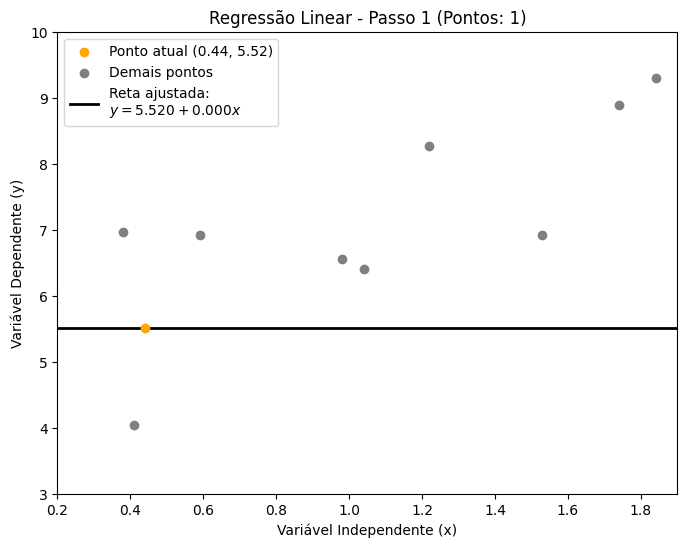
\includegraphics[scale=0.5]{figuras/RL_step_1.png}
	\end{center}
	\fonte{Autor.}
\end{figure}

Passo 2: Adiciona-se (1.74, 8.89)
\\ \\
n=2

\begin{gather*}
	\bar{x} = \frac{0.44 + 1.74}{2} = 1.09, \quad \bar{y} = \frac{5.52 + 8.89}{2} = 7.205
\end{gather*}

\begin{align*}
	\sum (x_i - \bar{x})(y_i - \bar{y}) &= \\
	(0.44 - 1.09)(5.52 - 7.205) + (1.74 - 1.09)(8.89 - 7.205) &=\\
	(-0.65)(-1.685) + (0.65)(1.685) &= \\
	1.09525 + 1.09525 &= 2.1905
\end{align*}

\begin{align*}
	\sum (x_i - \bar{x})^2 &=\\ 
	(0.44 - 1.09)^2 + (1.74 - 1.09)^2 &=\\
	0.4225 + 0.4225 &= 0.845
\end{align*}

\begin{gather*}
	\beta_0 = \frac{2.1905}{0.845} \approx 2.5923, \quad \beta_1 = 7.205 - 2.5923 \cdot 1.09 \approx 4.3795\\ \\
	\hat{y} = 4.3795 + 2.5923x
\end{gather*}

\begin{figure}[H]
	\caption{\label{fig:mqo_2}Passo 2 da regressão linear pelo método MQO.}
	\begin{center}
		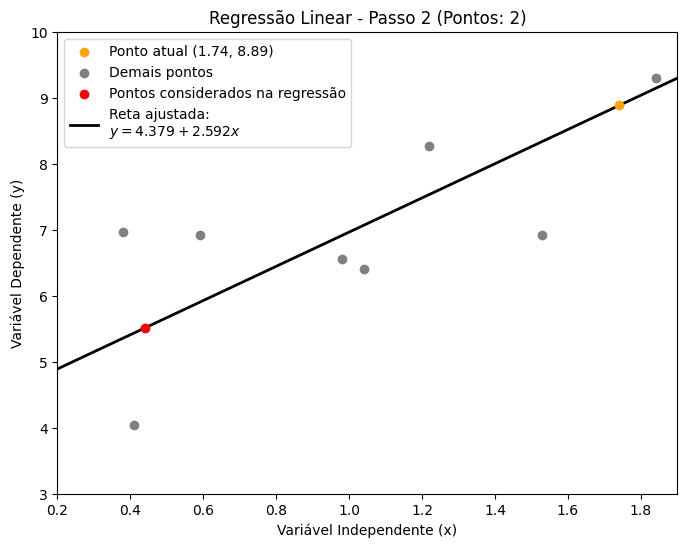
\includegraphics[scale=0.5]{figuras/RL_step_2.png}
	\end{center}
	\fonte{Autor.}
\end{figure}

Passo 3: Adiciona (0.41, 4.05)
\\ n = 3

\begin{gather*}
	\bar{x} = \frac{0.44 + 1.74 + 0.41}{3} = 0.8633, \quad \bar{y} = \frac{5.52 + 8.89 + 4.05}{3} = 6.1533 \\
	\sum (x_i - \bar{x})(y_i - \bar{y}) = \\ 
	(0.44 - 0.8633)(5.52 - 6.1533) + \\
	(1.74 - 0.8633)(8.89 - 6.1533) + \\
	(0.41 - 0.8633)(4.05 - 6.1533) \approx  \\
	0.268 + 2.399 + 0.953 = 3.62 \\ \\
	\sum (x_i - \bar{x})^2 = (0.44 - 0.8633)^2 + (1.74 - 0.8633)^2 + (0.41 - 0.8633)^2 \\
	\approx 0.179 + 0.769 + 0.205 = 1.153 \\
	\beta_0 = \frac{3.62}{1.153} \approx 3.1402 \\
	\beta_1 = 6.1533 - 3.1402 \cdot 0.8633 \approx 6.1533 - 2.711 = 3.4423 \\ \\
	\hat{y} = 3.4423 + 3.1402x
\end{gather*}

\begin{figure}[H]
	\caption{\label{fig:mqo_2}Passo 3 da regressão linear pelo método MQO.}
	\begin{center}
		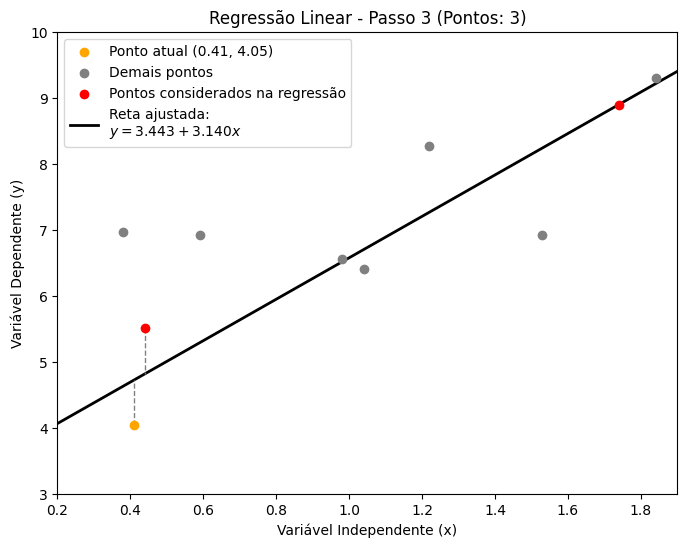
\includegraphics[scale=0.5]{figuras/RL_step_3.png}
	\end{center}
	\fonte{Autor.}
\end{figure}

Para os demais passos, o mesmo cálculo é realizado, onde a média amostral e os coeficientes são recalculados a cada iteração, conforme os pontos são adicionados.

\begin{figure}[H]
	\centering
	\caption{Iterações da aplicação do método MQO}
	\begin{subfigure}{0.4\textwidth}
	  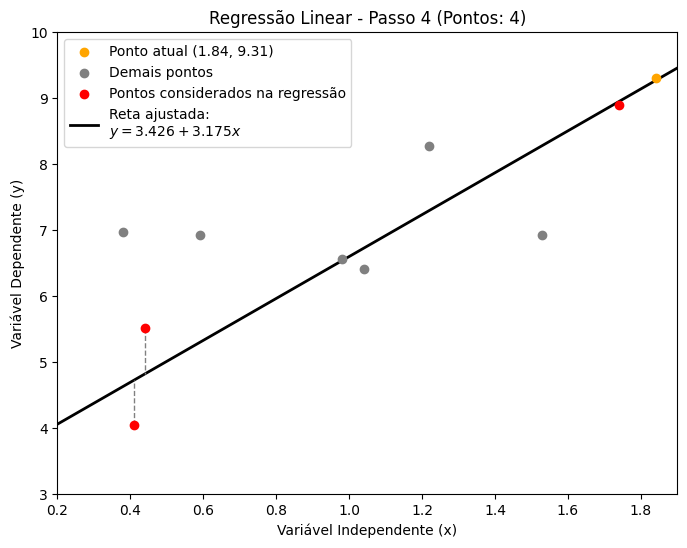
\includegraphics[width=\linewidth]{figuras/RL_step_4.png}
	  \caption{$n = 4$ | $y = 3,426 + 3,175x$}
	  \label{fig:mqo_4}
	\end{subfigure}
	\hspace{0.5cm}
	\begin{subfigure}{0.4\textwidth} 
		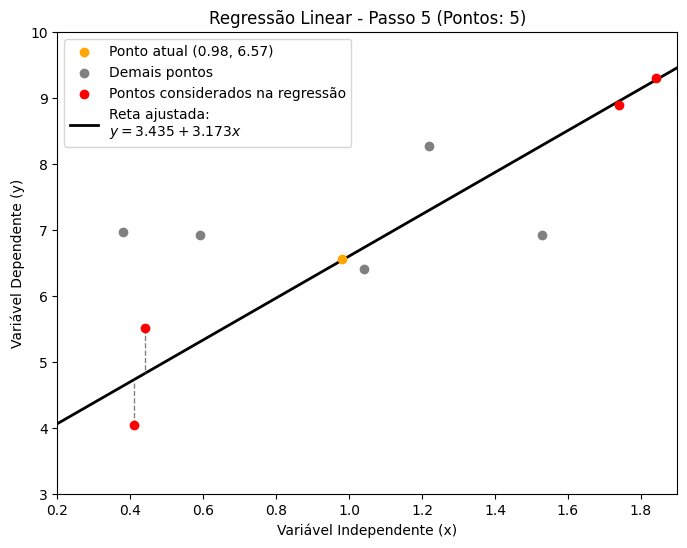
\includegraphics[width=\linewidth]{figuras/RL_step_5.png}
		\caption{$n = 5$ | $y = 3,435 + 3,173x$}
		\label{fig:intervalo_aplicacao_rls}
	\end{subfigure}
	\label{fig:mqo_5}
	\begin{subfigure}{0.4\textwidth} 
		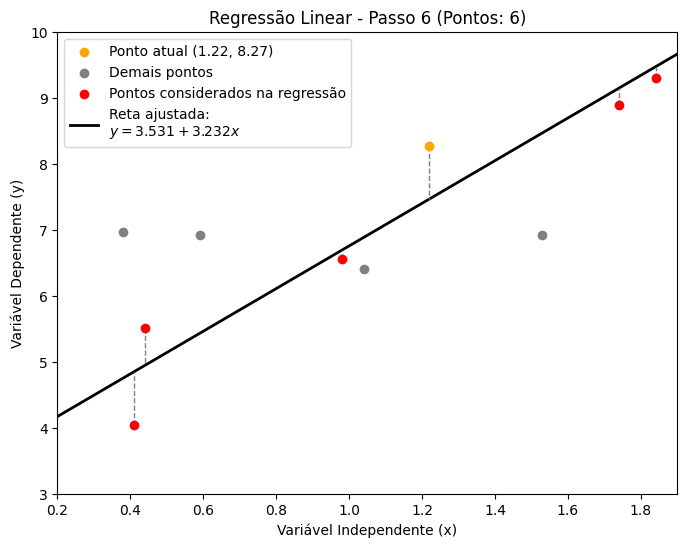
\includegraphics[width=\linewidth]{figuras/RL_step_6.png}
		\caption{$n = 6$ | $y = 3,531 + 3,232x$}
		\label{fig:intervalo_aplicacao_rls}
	\end{subfigure}
	\label{fig:mqo_6}
	\begin{subfigure}{0.4\textwidth} 
		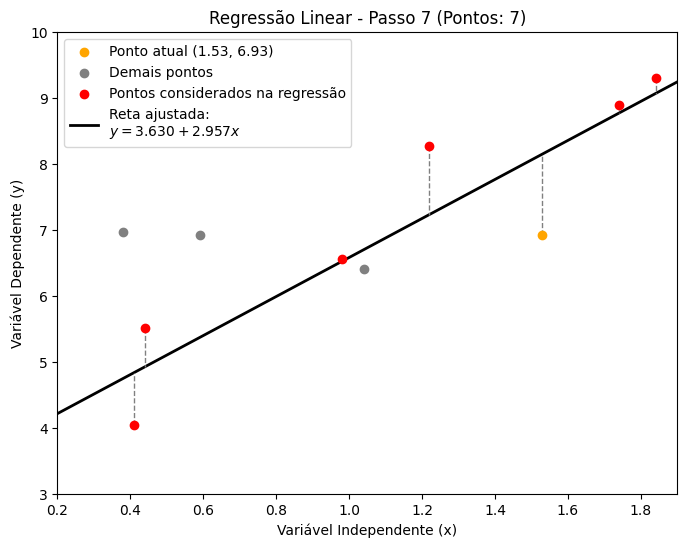
\includegraphics[width=\linewidth]{figuras/RL_step_7.png}
		\caption{$n = 7$ | $y = 3,630 + 2,957x$}
		\label{fig:intervalo_aplicacao_rls}
	\end{subfigure}
	\label{fig:mqo_7}
	\begin{subfigure}{0.4\textwidth} 
		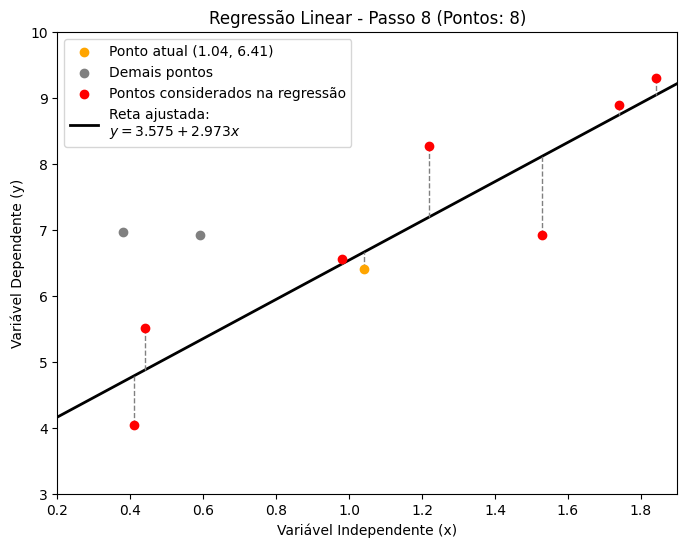
\includegraphics[width=\linewidth]{figuras/RL_step_8.png}
		\caption{$n = 8$ | $y = 3,575 + 2,973x$}
		\label{fig:intervalo_aplicacao_rls}
	\end{subfigure}
	\label{fig:mqo_8}
	\begin{subfigure}{0.4\textwidth} 
		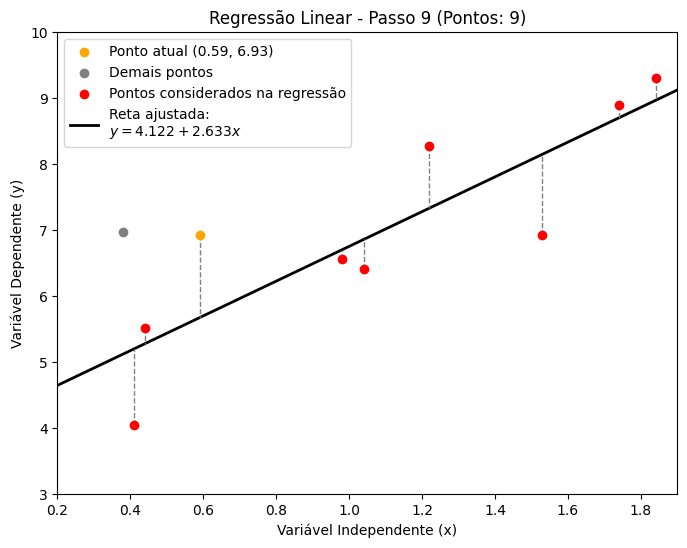
\includegraphics[width=\linewidth]{figuras/RL_step_9.png}
		\caption{$n = 9$ | $y = 4,122 + 2,633x$}
		\label{fig:intervalo_aplicacao_rls}
	\end{subfigure}
	\label{fig:mqo_9}
	\fonte{Autor.}
\end{figure}

Assim, a cada ponto selecionado da amostra, é calculada a derivada parcial da função estimada, determinando novos coeficientes que melhor descrevem a reta entre as amostras. Dado que não é possível estimar uma reta que passe sobre todos os pontos amostrados, os resíduos representados pelas linhas tracejadas na Figura \ref{fig:mqo_10} são definidos de tal modo que o somatório dos seus quadrados seja o menor possível.


\begin{figure}[H]
	\caption{\label{fig:mqo_10}Passo 10 da regressão linear pelo método MQO.}
	\begin{center}
		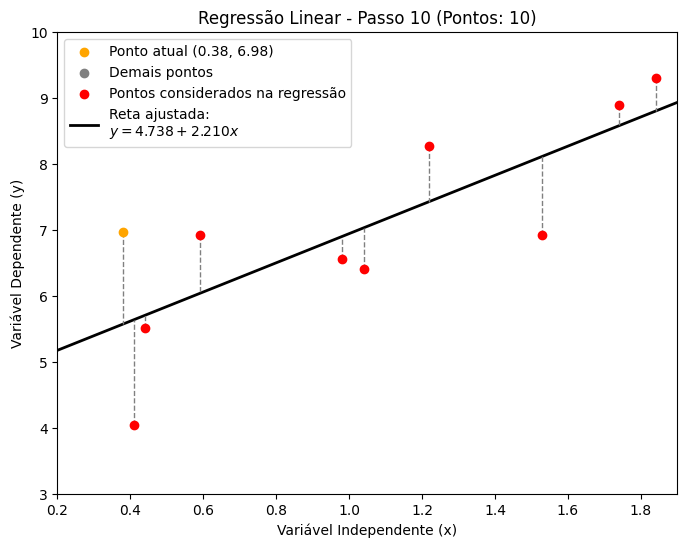
\includegraphics[scale=0.6]{figuras/RL_step_10.png}
	\end{center}
	\fonte{Autor.}
\end{figure}


\section{Modelo Ridge}
\label{sec:regressao-ridge}

A Regressão Ridge é uma técnica de regularização estatística amplamente utilizada em modelos de regressão linear para abordar problemas de sobreajuste (ou \textit{overfitting}, quando o modelo se ajusta demais aos dados de treinamento, perdendo a capacidade de prever dados fora da base passada para o modelo) e multicolinearidade entre variáveis preditoras \cite{McDonald:2009:RR}. Essa técnica, também conhecida como regularização L2, é particularmente eficaz em cenários onde o número de variáveis preditoras é grande ou quando essas variáveis apresentam alta correlação, o que pode levar a estimativas de coeficientes instáveis e de baixa generalização.

Conforme visto em \ref{sec:regressao-linear}, na regressão linear tradicional, o objetivo é minimizar o valor de \gls{RSS}, que mede a diferença entre os valores observados e os valores previstos pelo modelo. A função de perda é dada por:

\begin{equation}
	RSS = \sum_{i=1}^{n} (y_i - \hat{y}_i)^2
\end{equation}
\\

\noindent onde $y_i$ são os valores observados, $\hat{y}_i$ são os valores previstos, e $n$ é o número de observações. No entanto, em cenários com multicolinearidade (alta correlação entre variáveis preditoras) ou um grande número de preditores, o modelo pode se ajustar excessivamente aos dados de treinamento, resultando em alta variância e baixa performance em dados não vistos. A Regressão Ridge trata esse problema ao adicionar um termo de penalidade à função de perda, proporcional à soma dos quadrados dos coeficientes de regressão. 

A função objetivo da Regressão Ridge é:

\begin{equation}
	RSS_{L2} = \sum_{i=1}^{n} (y_i - \hat{y}_i)^2 + \alpha \sum_{j=1}^{p} \beta_j^2
\end{equation}

No contexto da biblioteca \textit{Scikit-learn} em Python, a classe Ridge implementa a Regressão Ridge. O parâmetro \textit{alpha} define a força da regularização: valores maiores de $\alpha$ resultam em coeficientes mais próximos de zero, enquanto valores menores permitem que o modelo se aproxime da regressão linear ordinária. A escolha adequada de 
$\alpha$ é crucial para evitar tanto o \textit{overfitting} quanto o \textit{underfitting} (quando o modelo é muito simples para capturar os padrões dos dados). \cite{ScikitLearnRidge2025}.

Além de impactar a função RSS, a Regressão Ridge altera o processo de busca pelos coeficientes $\beta$ que definem a reta (ou hiperplano, no caso de múltiplas variáveis) que melhor representa a regressão.

Na regressão linear tradicional, os coeficientes $\beta$ são encontrados minimizando-se apenas a soma dos quadrados dos resíduos, resultando em uma solução exata obtida pela equação normal:

\begin{equation}
	\hat{\boldsymbol\beta} = (\mathbf{X}^\top \mathbf{X})^{-1} \mathbf{X}^\top \mathbf{y}
\end{equation}

\noindent onde $\mathbf{X}$ é a matriz de variáveis independentes e $\mathbf{y}$ é o vetor de variáveis dependentes \cite{montgomery2012}.

Entretanto, quando há multicolinearidade ou grande número de variáveis, a matriz $\mathbf{X}^\top \mathbf{X}$  pode se tornar quase singular, causando coeficientes instáveis e de grande magnitude. A Regressão Ridge resolve isso ao adicionar o termo de penalização $\alpha \sum_{j=1}^{p}\beta_{j}^2$, modificando a equação normal para:

\begin{equation}
	\hat{\boldsymbol\beta}_{ridge} = (\mathbf{X}^\top \mathbf{X} + \alpha \mathbf{I})^{-1} \mathbf{X}^\top \mathbf{y}
\end{equation}

\noindent \cite{ScikitLearnRidge2025}.

Geometricamente, a regularização imposta pela Ridge faz com que a busca pela solução deixe de se restringir apenas à reta ou hiperplano definido pelo menor erro de previsão. Em vez disso, a solução passa a ser buscada dentro de uma região esférica ao redor da origem, delimitada pela penalização L2.

Com isso, mesmo que múltiplas combinações de coeficientes possam gerar ajustes semelhantes aos dados (especialmente em casos de multicolinearidade), a regressão \textit{Ridge} prefere aquelas soluções onde os coeficientes são menores, evitando oscilações extremas.

Portanto, o modelo \textit{Ridge} não apenas minimiza o erro de ajuste aos dados da \gls{RSS}, mas também impõe um “encolhimento” dos coeficientes em direção ao zero, resultando em retas ou hiperplanos mais estáveis, com menor variância e melhor capacidade de generalização para dados não vistos ao qual se deseja ser previsto \cite{McDonald:2009:RR}. \hl{Desse modo, devido a multicolinearidade entre as variáveis independentes, como temperatura, precipitação e níveis dos rios afluentes, a regularização L2 do modelo ajuda a estabilizar os coeficientes, reduzindo o risco de sobreajuste em cenários de alta variabilidade climática.}